\subsection{Recap: Code Scattering and Tangling}
\begin{frame}[fragile]{\myframetitle}
	\small\begin{mycolumns}[columns=3,T,animation=none,widths={43,32}]
\begin{codetight}{}
public class Graph {
	List nodes = new ArrayList();
	List edges = new ArrayList();

	Edge add(Node n, Node m) {
		Edge e = new Edge(n, m);
		nodes.add(n); nodes.add(m); edges.add(e);
		e.weight = new Weight();
		return e;
	}
	Edge add(Node n, Node m, Weight w) {
		Edge e = new Edge(n, m);
		nodes.add(n); nodes.add(m); edges.add(e);
		e.weight = w;
		return e;
	}
	void print() {
		for (int i = 0; i < edges.size(); i++) {
			((Edge) edges.get(i)).print();
		}
	}
}
\end{codetight}
		\mynextcolumn
\begin{codetight}{}
public class Node {
	int id = 0;
	Color color = new Color();

	void print() {
		Color.setDisplayColor(color);
		System.out.print(id);
	}
}
\end{codetight}
\begin{codetight}{}
public class Edge {
	Node a, b;
	Weight weight = new Weight();

	Edge(Node a, Node b) {
		this.a = a; this.b = b;
	}
	void print() {
		a.print(); b.print();
		weight.print();
	}
}
\end{codetight}
		\mynextcolumn
\begin{codetight}{}
public class Color {
	static void setDisplayColor(Color c) {...}
}
\end{codetight}	
\begin{codetight}{}
public class Weight {
	void print() {...}
}
\end{codetight}
		\hspace{10mm}
		\begin{note}{What is \ldots}
			\setlength\leftmargini{3mm}
			\begin{itemize}
				\item<+-> code scattering? 
				\item<+-> code tangling? 
				\item<+-> feature traceability? 
			\end{itemize}
		\end{note}
	\end{mycolumns}
\end{frame}
% note to editors: it is on purpose that no feature traces are shown on this slide, as the students are supposed to trace features manually

% TODO example copied from Lecture 2.2 and modified, integrate changes again? ideally we would have this code somewhere and reference it (rather than copying it)
% TODO would be nice to avoid this example clone (below) by ignoring @ and ~ on certain slides/animations

\begin{frame}[fragile]{\myframetitle}
	\small\begin{mycolumns}[columns=3,T,animation=none,widths={43,32}]
\begin{codetight}{}
public class Graph {
	List nodes = new ArrayList();
	List edges = new ArrayList();

	Edge add(Node n, Node m) {
		Edge e = new Edge(n, m);
		nodes.add(n); nodes.add(m); edges.add(e);
		@e.weight = new Weight();@
		return e;
	}
	@Edge add(Node n, Node m, Weight w) {
		Edge e = new Edge(n, m);
		nodes.add(n); nodes.add(m); edges.add(e);
		e.weight = w;
		return e;
	}@
	void print() {
		for (int i = 0; i < edges.size(); i++) {
			((Edge) edges.get(i)).print();
		}
	}
}
\end{codetight}
		\mynextcolumn
\begin{codetight}{}
public class Node {
	int id = 0;
	~Color color = new Color();~

	void print() {
		~Color.setDisplayColor(color);~
		System.out.print(id);
	}
}
\end{codetight}
\begin{codetight}{}
public class Edge {
	Node a, b;
	@Weight weight = new Weight();@

	Edge(Node a, Node b) {
		this.a = a; this.b = b;
	}
	void print() {
		a.print(); b.print();
		@weight.print();@
	}
}
\end{codetight}
		\mynextcolumn
\begin{codetight}{}
~public class Color {
	static void setDisplayColor(Color c) {...}
}~
\end{codetight}	
\begin{codetight}{}
@public class Weight {
	void print() {...}
}@
\end{codetight}
		\pause
		\begin{note}{Is it a problem for \ldots}
			\setlength\leftmargini{4mm}
			\begin{enumerate}[(a)]
				\item single systems? 
				\item runtime variability? {\tiny\lectureruntime}
				\item clone-and-own? {\tiny\lecturecloneandown}
				\item conditional compilation? {\tiny\lecturefeatures}
			\end{enumerate}
		\end{note}
	\end{mycolumns}
\end{frame}

\subsection{The Feature Traceability Problem}
\begin{frame}{\myframetitle}
	\begin{mycolumns}[animation=none]
		\mydefinition{Recap: Feature Traceability}{Feature traceability is the ability to trace a feature throughout the software life cycle (i.e., from requirements to source code).}
		\myexample{Recap: Intuition on Feature Traceability}{find feature 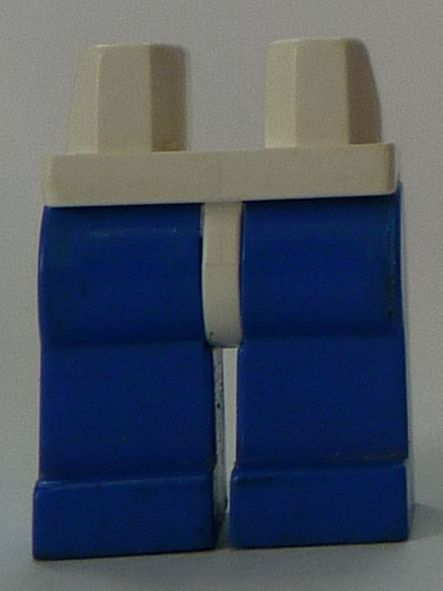
\includegraphics[width=.15\linewidth]{pants-blue} in product 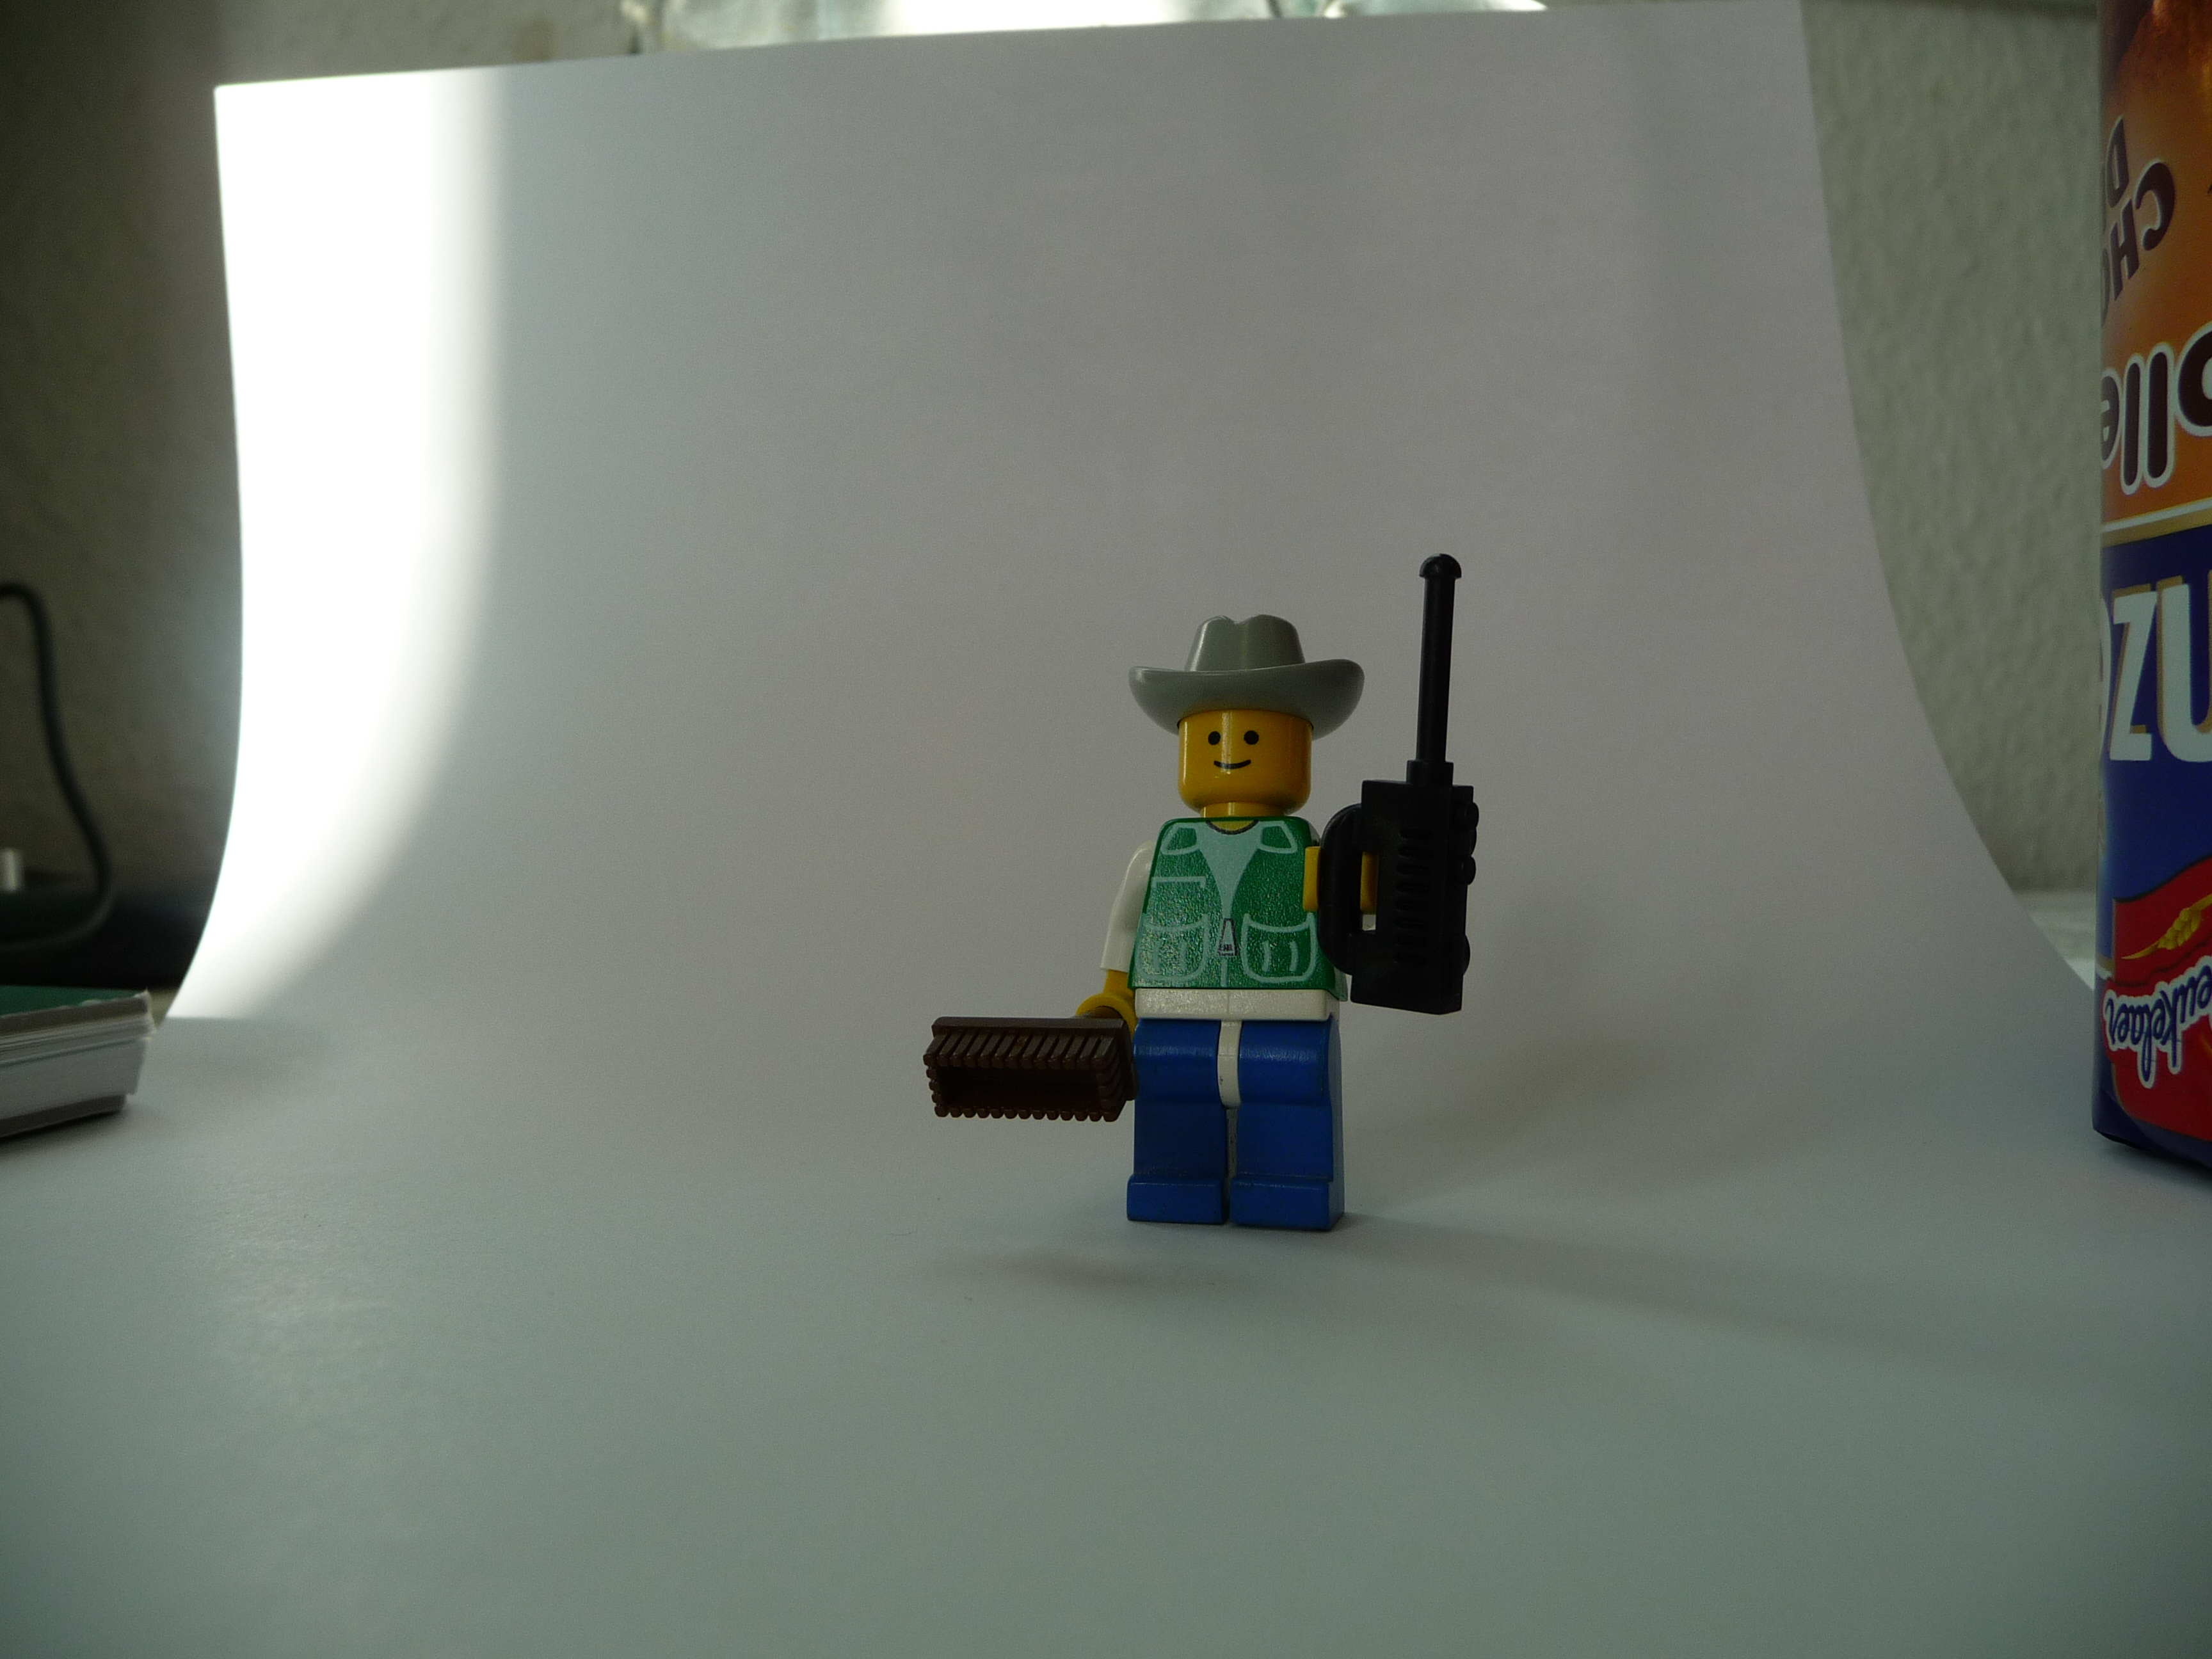
\includegraphics[width=.15\linewidth]{230}}
		\pause
		\mydefinition{Feature Traceability (revisited) \mysource{\fospl\mypage{54}}}{\mycite{Feature traceability is the ability to trace a feature from the \textbf{problem space} (for example, the feature model) to the \textbf{solution space} (that is, its manifestation in design and code artifacts).}}
	\mynextcolumn
		\pause\mydefinition{Feature Traceability Problem}{The feature traceability problem is the challenge to trace a feature in software artifacts (i.e., all or some locations).}
		\pause
		\centering\pic[width=.93\linewidth]{messy-lego}
	\end{mycolumns}
\end{frame}

%\subsection{Feature Location}
%\begin{frame}{\myframetitle}
%	\begin{mycolumns}
%		\todots
%	\mynextcolumn
%		\todots
%	\end{mycolumns}
%\end{frame}
% TODO add slide on feature location (in single system engineering)

\subsection{Feature Traceability with Colors}

\subsubsection*{Feature Commander}
\begin{frame}{\myframetitle}
	\begin{mycolumns}[animation=none,widths={35}]
		\begin{definition}{\featurecommander}
			\begin{itemize}
				\item each feature can be assigned to a color
				\item color used to support feature traceability
				\item features not assigned to a color shown in a shade of grade
				\item visualizations based on preprocessor macros % TODO check wording
			\end{itemize}
		\end{definition}
		\begin{note}{\href{https://www.tu-chemnitz.de/informatik/ST/research/material/xenomai/video.wmv}{Demo Video}}
			 (there is no sound)
		\end{note}
	\mynextcolumn
		\only<1,6-|handout:1>{\pic[width=\linewidth]{feature-commander1-cropped}}%
		\only<2|handout:0>{\pic[width=\linewidth,trim=0 450 600 0,clip]{feature-commander1-cropped}}%
		\only<3|handout:0>{\pic[width=\linewidth,trim=750 400 -150 50,clip]{feature-commander1-cropped}}%
		\only<4|handout:0>{\pic[width=\linewidth,trim=175 175 425 275,clip]{feature-commander1-cropped}}%
		\only<5|handout:0>{\pic[width=\linewidth,trim=600 0 0 450,clip]{feature-commander1-cropped}}%
	\end{mycolumns}
\end{frame}

\begin{frame}{\myframetitle}
	\begin{mycolumns}[animation=none,widths={65}]
		\only<1,5-|handout:1>{\pic[width=\linewidth]{feature-commander2-cropped}}%
		\only<2|handout:0>{\pic[width=\linewidth,trim=0 450 600 0,clip]{feature-commander2-cropped}}%
		\only<3|handout:0>{\pic[width=\linewidth,trim=600 450 0 0,clip]{feature-commander2-cropped}}%
		\only<4|handout:0>{\pic[width=\linewidth,trim=600 0 0 450,clip]{feature-commander2-cropped}}%
	\mynextcolumn
		\begin{definition}{\featurecommander}
			\begin{itemize}
				\item research prototype (last update August 2010)
				\item only static view on the source code
				\item only works for \href{https://source.denx.de/Xenomai/xenomai/-/wikis/home}{Xenomai} (a real-time core for Linux)
				\item further reading on experiments with developers: \backgroundcolors
			\end{itemize}
		\end{definition}
	\end{mycolumns}
\end{frame}

\subsubsection*{FeatureIDE}
\begin{frame}{\myframetitle}
	\begin{mycolumns}[animation=none,widths={65}]
		\only<1,4-|handout:1>{\pic[width=\linewidth]{feature-traceability}}%
		\only<2|handout:0>{\pic[width=\linewidth,trim=0 160 350 120,clip]{feature-traceability}}%
		\only<3|handout:0>{\pic[width=\linewidth,trim=210 65 140 295,clip]{feature-traceability}}%
	\mynextcolumn
		\begin{definition}{FeatureIDE\mysource{\featureide}}
			\begin{itemize}
				\item tool support for feature traceability
				\item inspired by Feature~Commander
				\item color can be assigned to features
				\item colors used in feature model, configurations, package explorer, and source code
			\end{itemize}
		\end{definition}
		\begin{note}{\href{https://youtu.be/jVe7f32mLCQ?t=240}{Demo Video} (last minute only)}
			\begin{itemize}
				\item collaboration view
				\item support for colors
			\end{itemize}
		\end{note}
	\end{mycolumns}
\end{frame}
% \href{https://www.youtube.com/watch?v=S32Cy2LXB8o}{assigning colors from everywhere}
% \href{https://www.youtube.com/watch?v=9QNDu0rMuQQ}{overview on support for colors with FeatureHouse (even in generated code)}

\subsection{Virtual Separation of Concerns}
\begin{frame}{\myframetitle\mysource{\virtualseparation}}
	\begin{mycolumns}
		\begin{definition}{Virtual Separation of Concerns}
			\begin{itemize}
				\item annotations of code based on the underlying structure (i.e., abstract syntax)
				\item \textbf{disciplined annotations}: only optional nodes in the abstract syntax tree can be annotated
				\item tool support used to provide views and navigate in source code
				\item \textbf{syntactic correctness} guaranteed for all generated program variants
			\end{itemize}
		\end{definition}
		% TODO show abstract syntax tree here? maybe for expressions with addition, multiplication, and values. or classes, class name, methods, fields, parameters, return type?
	\mynextcolumn
		\begin{note}{What is different with preprocessors?}
			\begin{itemize}
				\item annotation of characters in plain text
				\item undisciplined annotations possible
				\item can lead to generation of syntactically invalid program variants
			\end{itemize}
		\end{note}
		\begin{note}{What is different with physical separation?}
			\begin{itemize}
				\item features physically separated from each other
				\item dedicated components, services, plug-ins \lecturemodules
				\item dedicated modules, folders, files \lecturelanguages
			\end{itemize}
		\end{note}
	\end{mycolumns}
\end{frame}

\subsubsection*{CIDE}
\begin{frame}{\myframetitle\mysource{\cide}}
	\begin{mycolumns}[widths={60},animation=none]
		\pic[width=\linewidth]{cide-open-editor}
	\mynextcolumn
		\begin{example}{What is CIDE?}
			\begin{itemize}
				\item stands for Colored Integrated Development Environment
				\item colors used to mark features
				\item based on Eclipse~3.5 and FeatureIDE
				\item research prototype (last update in May 2012)
				\item special editors available for several languages:
				ANTLR, Bali, C (experimental), C++ (experimental), C\#, ECMAScript (JavaScript), Featherweight Java, \textbf{Java 1.5}, gCIDE, Haskell, HTML, JavaCC, OSGi Manifest, Properties, Python, and XHTML
			\end{itemize}
		\end{example}
	\end{mycolumns}
\end{frame}
%Featherweight Java 	.fj 	
%Java 	.java 	
%Java (JDT) 	.java 	recommended, supports type checking
%C 	.c, .h 	exact parser, does not understand preprocessor statements
%C (approx) 	.c, .h 	pseudo-parser, does not recognize full structure and not all preprocessor statements; use only one C extension at a time
%C# 	.cs 	
%ECMAScript (JavaScript) 	.js 	
%Haskell 	.hs 	pseudo-parser, skips over expressions
%Bali 	.b 	supports type checking
%ANTLR 	.g 	simple productions only, no options or semantic extensions.
%JavaCC 	.cc 	
%gCIDE 	.gcide 	bootstrapped grammar for gCIDE itself
%Properties 	.properties 	for line-based property files
%HTML and XML 	.html; .xml 	XML parser does not parse doctype declarations yet (not compatible with Eclipse's WST plugins for some reason)
%XHTML 	.xhtml 	version 1.0 strict, does not understand doctype declaration yet; generated from dtd
%XML-People 	.xml 	simple proof-of-concept parser for the following DTD: [people.dtd]; do not use together with XML extension
%Python 	.py 	
%OSGi Manifest 	MANIFEST.MF 	simple, with simple type system

\begin{frame}{\myframetitle\mysource{\cide}}
	\begin{mycolumns}[widths={70},animation=none]
		\pic[width=\linewidth]{cide-editor-and-outline}
	\mynextcolumn
		\begin{example}{Why colors?}
			\begin{itemize}
				\item colors replace preprocessor directives
				\item features relevant for development task are assigned a color
				\item code annotated to a feature by selection and context menu
				\item features visualized by background colors
				\item annotations stored externally (no changes outside the special editor feasible)
			\end{itemize}
		\end{example}
	\end{mycolumns}
\end{frame}

\begin{frame}{\myframetitle\mysource{\cide}}
	\begin{mycolumns}[widths={65},animation=none]
		\pic[width=\linewidth]{cide}
	\mynextcolumn
		\begin{example}{Why virtual separation?}
			\begin{itemize}
				\item source code is a view on the abstract syntax tree (AST)
				\item possible to hide irrelevant features
				\item possible to show overlapping features
				\item supporting development despite scattering and tangling
				\item no need to handle separators and logical connectors:\\\mycite{\texttt{,}}, \mycite{\texttt{||}}
				\item efficient detection of type errors \lectureanalyses
			\end{itemize}
		\end{example}
	\end{mycolumns}
\end{frame}

\begin{frame}{\myframetitle\mysource{\cide}}
	\pic[width=\linewidth]{cide-show-single-feature}
	\begin{example}{}\centering
		\textbf{view on a feature}: possible to only show a single feature -- in its surrounded code
	\end{example}
\end{frame}

\begin{frame}{\myframetitle\mysource{\cide}}
	\begin{mycolumns}[widths={45},animation=none]
		\begin{example}{Why configuration?}
			\begin{itemize}
				\item features specified in FeatureIDE feature model
				\item configuration created in FeatureIDE configuration editor
				\item configuration used to generate and visualize variant
				\item \ldots
			\end{itemize}
		\end{example}
	\mynextcolumn
		\pic[width=\linewidth]{cide-feature-selection}
	\end{mycolumns}
\end{frame}

\begin{frame}{\myframetitle\mysource{\cide}}
	\begin{mycolumns}[widths={45},animation=none]
		\begin{example}{Why configuration?}
			\begin{itemize}
				\item \ldots
				\item \textbf{view on a variant}: variant visualized in source code and project explorer
				\item only necessary to press CIDE button in project explorer
				\item pressing it again returns to the view of the product line
			\end{itemize}
		\end{example}
	\mynextcolumn
		\pic[width=\linewidth]{cide-variant-view-in-project-explorer}
	\end{mycolumns}
\end{frame}
% CIDE literature
% forward reference to physical separation of concerns in next two lectures
